\section{Opgaver}
\begin{opgave}{Neutrinoernes vilde verden}
    Med udgangspunkt i afsnit \ref{sec:lepton} navngiv på alle neutrinoerne:
    \begin{itemize}
        \item $\nu_\mathrm{e}$
        \item $\nu_\mu$
        \item $\nu_\tau$
        \item $\bar{\nu}_\mathrm{e}$
        \item $\bar{\nu}_\mu$
        \item $\bar{\nu}_\tau$
    \end{itemize}
    ~
    \opg Forklar hvorfor neutrinoer er så svære at måle eksperimentelt.
    \opg Hvilke(n) bevarelseslov(e) er antielektronneutrinoen i $\beta^-$-henfaldet, figur \ref{fig:betaminus}, nødvendig for at reaktionen opfylder?
\end{opgave}

\begin{opgave}{Leptonfamilier}
    \opg Hvilke leptoner tilhører myonfamilien?
    \opg Hvordan adskiller myonfamilien sig fra elektronfamilien?
    \opg Hvilken familie er mest stabil og hvorfor?
\end{opgave}

\begin{opgave}{Kvarksammensætning}
    Hvordan kan man sammensætte tre kvarker af første generation, således at partiklen bliver elektrisk neutral (har elektrisk ladning $q=0$)?
\end{opgave}

\begin{figure}
    \centering
    \begin{tikzpicture}
    \vertex{0,0};
        \draw[fermion] (-1.5,0) node[anchor = east]{$\mathrm{e}^-$} -- (0,0);
        \draw[photon] (0,0) -- (1.5,1) node[anchor = south west]{$\gamma$};
        \draw[fermion] (0,0) -- (1.5,-1)node[anchor = north west]{$\mathrm{e}^-$};
    \end{tikzpicture}
    \caption{$\gamma$-henfald af en eksiteret elektron.}
    \label{fig:gamma}
\end{figure}


\begin{opgave}{$\mathbf{\gamma}$-henfald af atomer}
    Nogle gange sker det at atomer har så meget energi at de udsender lys i form af en foton, hvilket kaldes et $\gamma$-henfald. Dette kan beskrives med Feynmandiagrammet i figur \ref{fig:gamma}.
    \opg Foregår reaktionen gennem en elektromagnetisk, stærk eller svag vekselvirkning? \\
    \textit{Hint: Hvilken boson er tegnet i diagrammet?}
    \opg Hvilken type vekselvirkning står for $\beta^-$-henfaldet i figur \ref{fig:betaminus}?
    \opg Protoner har kvarksammensætningen uud, mens neutronen har kvarksammensætningen udd. Tegn Feynmandiagrammet for reaktionen med alle kvarker i stedet for blot en proton og en neutron.
    \opg Ved $\beta^+$-henfald omdannes en proton, p, til en neutron, n, en positron, e$^+$, og en elektronneutrino, $\nu_\mathrm{e}$. Tegn Feynmandiagrammet for dette henfald.
    \opg Sammenlig Feynmandiagrammet for $\beta^-$- og $\beta^+$-henfaldene. \\
    \textit{Hint: Figurene \ref{fig:vertex_rot_el} og \ref{fig:vertex_rot_svag}.}
\end{opgave}

\begin{opgave}{Bevarelseslove}
    \opg Kig på følgende reaktioner og bestem, om de kan lade sig gøre eller ej.
    \begin{enumerate}
        \item $\mathrm{e}^- \longleftrightarrow \mathrm{e}^- + \mathrm{e}^+ + \mathrm{e}^+$
        \item $\mathrm{p} + \mathrm{n} \longleftrightarrow \mathrm{e}^- + \mathrm{e}^+ + \mathrm{e}^+$
        \item $\mathrm{p} + \mathrm{n} + \mathrm{e}^+ \longleftrightarrow \mathrm{n} + \mathrm{p} + \bar{\nu}_\mathrm{e}$
        \item $\mathrm{p} \longleftrightarrow \mu^- + \mathrm{n} + \bar{\nu}_\mu $
        \item $\mathrm{p} \longleftrightarrow \mu^+ + \mathrm{n} + \nu_\mu $
        \item $\bar{\mathrm{n}} \longleftrightarrow \bar{\mathrm{p}} + \mathrm{e}^+ + \nu_\mathrm{e}$
        \item $\mathrm{e}^- + \mu^+ \longleftrightarrow \text{n}$
    \end{enumerate}
    \emph{Hint: tjek om bevarelseslovene er opfyldt.}
\end{opgave}

\newpage

\begin{opgave}{Dannelse af myoner}
    Myoner kan dannes ud fra en foton. Reaktionsskemaet for reaktionen er
    %
    \begin{align}
        \gamma \rightarrow \mu^- + x
    \end{align}
    %
    hvor $x$ er en anden elementarpartikel.
    \opg Hvilken partikel skal det være, for at opfylde bevarelseslovene som angivet i afsnit \ref{sec:partikelreaktioner}?
    \opg Tegn et Feynmandiagram for reaktionen.
\end{opgave}

\begin{opgave}{Rotation af knudepunkter i Feynmandiagrammer} \label{opg:rotation_af_Feynman}
    Betragt reaktionen i Figur \ref{fig:Wvertex}.
    \begin{figure}[h]
        \centering
        \begin{tikzpicture}
            \draw[fermion] (-1,0) node[anchor = east]{$\nu_\mathrm{e}$} -- (0,0);
            \draw[boson] (0,0) -- (1,1)node[anchor = west]{$\mathrm{W}^+$};
            \draw[fermion] (0,0) --(1,-1)node[anchor = west]{$\mathrm{e}^-$};
            \vertex{0,0};
        \end{tikzpicture}
        \caption{Udsendelse af en $\mathrm{W}^+$-boson.}
        \label{fig:Wvertex}
    \end{figure}
    \opg Rotér Feynmandiagrammet mod uret, så det viser en indkommende positron i stedet. Hvilken slags neutrino produceres der?
    \opg Hvad er ladningen af $\mathrm{W}$-bosonen nu?
    \opg Udskift positronen med en elektron. Hvilken slags neutrino produceres der?
    \opg Hvad er ladningen af $\mathrm{W}$-bosonen nu?
    \opg Forklar hvorfor de to Feynmandiagrammer i figur \ref{fig:annihilation_pardannelse} tilsyneladende kan roteres \SI{180}{\degree} uden at skifte ladningernes fortegn, modsat af hvad som for rotation af knudepunkter kræver.
\end{opgave}

\begin{opgave}{Kvarkkobling}
    Kvarkerne kobler til hinanden gennem den svage vekselvirkning, eller sagt på en anden måde kan den svage kernekraft omdanne en kvark til en anden, se figur \ref{fig:vertex}.  Figur \ref{fig:kvarkkobling} viser en oversigt over kvarkerne, hvor pilen mellem u- og d-kvarken betyder, at $\mathrm{W}$-bosonen kan ændre disse kvarker til hinanden. 
    \begin{figure}[h!]
        \centering
        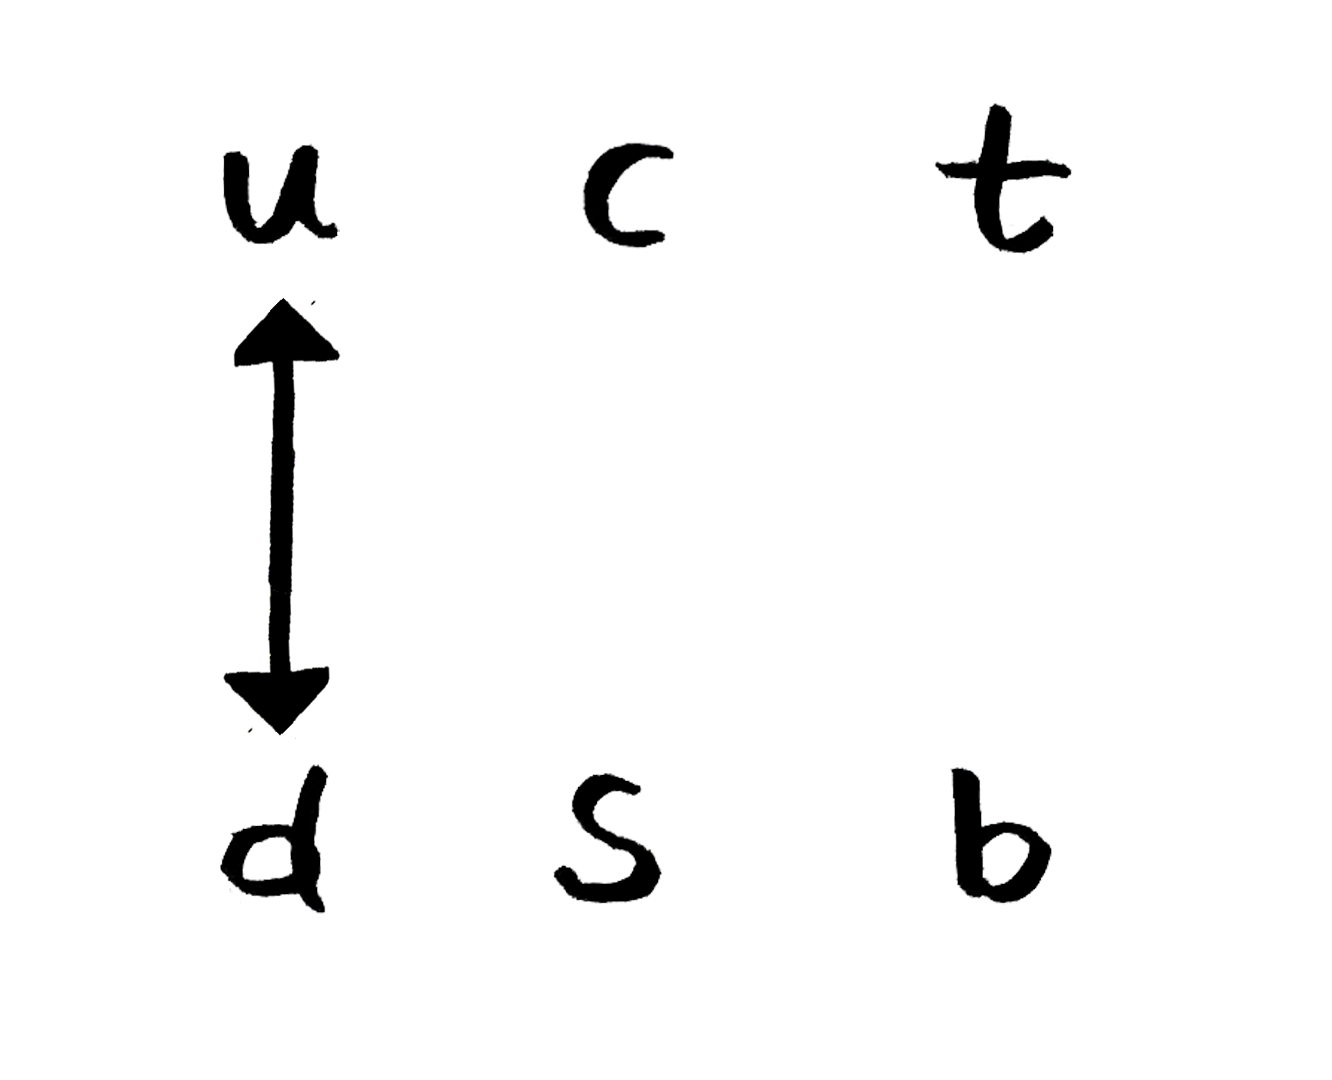
\includegraphics[width=0.3\textwidth]{Partikel/figurer/kvarkkobling.png}
        \caption{$\mathrm{W}$-bosonen kan ændre kvarker til en anden type så længe ladningen ændres med $\pm 1$}
        \label{fig:kvarkkobling}
    \end{figure}
    \opg Tegn en kopi af figur \ref{fig:kvarkkobling} med pile mellem alle de kvarker, som $\mathrm{W}$ kobler. 
    \opg En t-kvark omdannes til en b-kvark under udsendelse af en $\mathrm{W}$-partikel. Tegn Feynmandiagrammet.
    \opg Hvad er ladningen af $\mathrm{W}$?
    \opg En s-kvark og en anti-c kvark annihilerer og skaber en $\mathrm{W}$-partikel. Tegn Feynmandiagrammet.
    \opg Hvad er ladningen af $\mathrm{W}$?
    \opg Er W-bosonen stabil, og hvis ikke hvad henfalder den til? Indtegn i sidste tilfælde dette i Feynmandiagrammet.
\end{opgave}

\begin{opgave}{Feynman-diagrammer: En sand kunstart} \label{opg:feynman1}
    Gluonen, som bærer den stærke vekselvirkning, virker ved at ændre kvarkernes farveladning. Feltet som beskæftiger sig med dette kaldes for kvantekromodynamik\footnote{Kromo er den danske stavemåde af det græske "chromo",~der betyder farve.}. Kvantekromodynamik er dog en anelse\footnote{Kun lidt ironisk.} ud over niveauet for denne camp, men det forhindrer os ikke i at gøre brug af gluonen i vores Feynmandiagrammer.
    \begin{figure} [h!]
        \centering
        \begin{tikzpicture}
            \draw[fermion] (0,0.25) node[anchor = east]{d}-- (2,1.5);
            \draw[fermion] (2,-1) -- (0,-0.25)node[anchor = east]{$\bar{\mathrm{c}}$};
            \draw[fermion] (6,-0.25) node[anchor=west]{$\bar{\mathrm s}$} -- (2,-1);
            \draw[fermion] (2,1.5) -- (6,2.25) node[anchor = west]{d};
            \draw[gluon] (2,1.5) -- (4,0.75);
            \draw (3,1) node[anchor = north east]{g};
            \draw[fermion] (6,1.75) node[anchor = west]{$\bar{\mathrm u}$} -- (4,0.75);
            \draw[fermion] (4,0.75) -- (6,0.25) node[anchor = west]{u};
            \draw[boson] (2,-1) -- (4,-2);
            \draw[fermion] (4,-2) -- (6,-1.75) node[anchor = west]{d};
            \draw[fermion] (6,-2.25) node[anchor = west]{$\bar{\mathrm u}$} -- (4,-2);
            \draw (3.2,-1.6) node[anchor = north east]{$\mathrm{W}^\pm$};
            \vertex{2,1.5};
            \vertex{2,-1};
            \vertex{4,0.75};
            \vertex{4,-2};
            \draw[line width = 0.5mm] (-0.25,-0.5) -- (-0.5,-0.5) -- (-0.5,0.5) -- (-0.25,0.5);
            \draw (-0.5,0) node[anchor = east]{$\mathrm{D}^-$};
            \draw[line width = 0.5mm] (6.25,-0.5) -- (6.5,-0.5) -- (6.5,0.5) -- (6.25,0.5);
            \draw[line width = 0.5mm] (6.25,1.5) -- (6.5,1.5) -- (6.5,2.5) -- (6.25,2.5);
            \draw[line width = 0.5mm] (6.25,-1.5) -- (6.5,-1.5) -- (6.5,-2.5) -- (6.25,-2.5);
            \draw (6.5,0) node[anchor = west]{$\mathrm{K}^+$};
            \draw (6.5,2) node[anchor = west]{$\pi^-$};
            \draw (6.5,-2) node[anchor = west]{$\pi^-$};
        \end{tikzpicture}
        \caption{Henfaldet af D$^-$-mesonen til K$^+$ og 2$\pi^-$.}
        \label{fig:quark_inter}
    \end{figure}
    
    \noindent Figur \ref{fig:quark_inter} viser et eksempel på en vekselvirkning hvor gluonen indgår. Kvarktypen ændrer sig ikke under udsendelse af en gluon (kun dens farve, men igen, det behøver vi ikke tage højde for). Gluonen henfalder til et vilkårligt kvark-antikvark-par Gluonens energi afgør, hvilket kvark-antikvarkpar, der kan dannes, men u- og d-kvarken er de mindst energirige (mindst masse) og kan derfor altid dannes med høj sandsynlighed. Det betyder, at det er ``gratis''  at introducere en gluon i sit Feynmandiagram, som enten henfalder til et u$\bar{\text{u}}$- eller d$\bar{\text{d}}$-par, hvilket kaldes en $\pi^0$-meson. \\

    Disse egenskaber kan bruges til forstå henfald af sammensatte partikler. Her kigges på henfaldet:
    \begin{equation*}
        \text{D}^- \rightarrow \text{K}^+ + \pi^- + \pi^-.
    \end{equation*}
    Dette er henfaldet af $\text{D}^-$-mesonen (kvarksammensætning: d$\bar{\text{c}}$ ) til mesonerne K$^+$ (u$\bar{\text{s}}$), og to $\pi^-$ (d$\bar{\text{u}}$). Et sådant henfald er vist i figur \ref{fig:quark_inter}. Læg mærke til, at man kan sætte klammer om de kvarker, der hører sammen i en partikel.
    Udfordringen består i at lave et Feynmandiagram, der er så overskueligt som muligt (f.eks. uden krydsende pile) og med \emph{så få knudepunkter, og derved så få virtuelle partikler, som muligt}. Fysisk set betyder færre knudepunkter at reaktionen har større sandsynlighed for at forekomme.
    \opg Hvad er ladningen af $\mathrm{W}$-bosonen i figur \ref{fig:quark_inter}?
    \opg Beskriv med ord hvad der sker med hver af kvarkerne i D$^-$-mesonen.
    \opg Prøv at lave et Feynmandiagram for henfaldet: $\text{D}^- \rightarrow \text{K}^- + \pi^+ + \pi^-$. \\
    \emph{Hint: start med at finde kvarksammensætningen af partiklerne.}
    \opg Er det mest sandsynligt at reaktionen danner mesonerne K$^+$ og $\pi^-$ eller K$^-$ og $\pi^+$ ud over den $\pi^-$-meson, der dannes i begge reaktioner?
\end{opgave}

\begin{opgave}{Flere Feynmandiagrammer} \label{opg:flere_feynman}
    Tegn Feynmandiagrammer for følgende henfald. Husk at gøre brug af så få knudepunkter som muligt.
    \opg $\text{B}^- (\mathrm b\bar{\mathrm u}) \longrightarrow \text{D}^0(\mathrm c\bar{\mathrm u}) + \rho^-(\mathrm d\bar{\mathrm u})$
    \opg $\Sigma^-(\mathrm{dds}) \longrightarrow \Lambda^0 (\mathrm{uds}) + \mathrm{e}^- + \bar{\nu}_\mathrm{e}$
    \opg $\Delta^0 (\mathrm{udd}) \longrightarrow \mathrm{p} + \pi^- (\mathrm d\bar{\mathrm u})$
    \opg $\text{D}_\mathrm{s}^+ (\mathrm c\bar{\mathrm s}) \longrightarrow \phi (\mathrm s\bar{\mathrm s}) + \rho^+ (\mathrm u\bar{\mathrm d})$
    \opg $\Omega^-(\mathrm{sss}) \longrightarrow \Xi^-(\mathrm{dss}) + \pi^0(\mathrm u\bar{\mathrm u})$
\end{opgave}

\begin{opgave}{Endnu flere Feynmandiagrammer}
    Betragt tre reaktioner
    \begin{align*}
        &1. \enspace \eta \rightarrow \pi^+ + \pi^- + \mathrm{e}^+ + \mathrm{e}^- \\
        &2. \enspace \tau^- \rightarrow \pi^0 + \pi^- + \nu_\tau \\
        &3. \enspace K^{*0} \rightarrow K^+ + \pi^- \\
        &4. \enspace K^+ \rightarrow \pi^+
    \end{align*}
    Her er kvarksammensætningen af mesonerne
    \begin{align*}
        \eta&: \enspace \mathrm u \bar{\mathrm u}, \mathrm d \bar{\mathrm d}, \mathrm s \bar{\mathrm s} \\
        \pi^+&: \enspace \mathrm u \bar{\mathrm d} \\
        \pi^0&: \enspace \mathrm u \bar{\mathrm u}, \mathrm d \bar{\mathrm d} \\
        \mathrm K^{*0}&: \enspace \mathrm d \bar{\mathrm{s}} \\
        \mathrm K^+&: \enspace \mathrm u \bar{\mathrm{s}}
        \end{align*}
    \opg $\pi^+$ og $\pi^-$ er hinandens antipartikler. Hvad er kvarksammensætningen af $\pi^-$?
    \opg Ved hvilken type vekselvirkning sker hvert henfald?
    \opg Tegn Feynmandiagrammer for henfaldene.
    \opg Hvor mange knudepunkter er der i de(t) henfald, der forekommer ved svag vekselvirkning?
    \opg Er der nogle reaktioner, der er så usandsynlig at den praktisk talt aldrig forekommer? \\
    \textit{Hint: Se afsnit \ref{sec:reaktionssandsynlighed}}.
\end{opgave}

\begin{figure}[h!]
    \centering
    \begin{tikzpicture}
		    \draw[fermion] (0,0) node[anchor = east]{u}-- (2,0);
            \draw[fermion] (2,0) -- (6,1) node[anchor = west]{u};
            \draw[gluon] (2,0) -- (4,-0.75);
            \draw (3,-0.5) node[anchor = north east]{g};
            \draw[fermion] (6,-0.5) node[anchor = west]{$\bar{\mathrm u}$} -- (4,-0.75);
            \draw[fermion] (4,-0.75) -- (6,-1.05) node[anchor = west]{u};
		    \vertex{2,0};
		    \vertex{4,-0.75};
            \draw[line width = 0.5mm] (6.25,-0.2) -- (6.5,-0.2) -- (6.5,-1.3) -- (6.25,-1.3);
            \draw (6.5,-.7) node[anchor = west]{$\pi^0$};
		\end{tikzpicture}
    \caption{Henfald af en højenergikvark ved udsendelse af en $\pi^0$.}
    \label{fig:u-henfald}
\end{figure}
\begin{opgave}{Reaktionssandsynlighed}
    En højenergikvark kan afgive noget af sin energi ved et udsende en neutral pion, $\pi^0$, gennem en virtuel partikel. Den neutrale pion består enten af kvarkerne u$\bar{\mathrm{u}}$ eller d$\bar{\mathrm{d}}$, hvilket betyder at reaktionen skal kunne danne begge kombinationer. For at gøre det konkret vælges en u-kvark.
    \opg I figur \ref{fig:u-henfald} ses en af de tre mulige måder hvorpå reaktionen kan forekomme. Foregår reaktionen ved en elektromagnetisk, stærk eller svag vekselvirkning?
    \opg Tegn Feynmandiagrammerne for reaktionen med de to andre vekselvirkninger.
    \opg Hvilke bosoner kan reaktionen ikke forekomme med som virtuel partikel?
    \opg Ranger reaktionerne efter hvor sandsynlige de er ud fra afsnit \ref{sec:reaktionssandsynlighed} og forklar dit ræsonnement.
    \opg Forklar at der i alle reaktioner også godt kan dannes kvarkparet d$\bar{\mathrm{d}}$ i stedet for u$\bar{\mathrm{u}}$, således at der faktisk er tale om en neutral pion.
\end{opgave}